\documentclass[a4paper, 11pt]{article}
\usepackage[left=2.5cm,right=2.5cm,top=3cm,bottom=3cm,a4paper]{geometry}
\usepackage{kotex}
\usepackage{color}
\usepackage{enumitem}
\usepackage[cmyk, dvipsnames, svgnames]{xcolor}
\usepackage{graphicx}
\DeclareGraphicsExtensions{.pdf,.png,.jpg}
\usepackage[onehalfspacing]{setspace}
\setstretch{2.0}
\usepackage[colorlinks,urlcolor=blue,filecolor=magenta]{hyperref}
\usepackage{url}






\title{\textbf{\Huge오목 한글 설명서}}
\author{\textbf{\LARGE5조}}
\begin{document}
	
	\maketitle
	
	\vspace{6cm}
	\begin{center}
		\textbf{\large20134824김민석}\\
		\textbf{\large20134852허정건}\\
		\textbf{\large20134867이현문}\\
	\end{center}
	
	
	
	
	\maketitle
	\newpage
	\thispagestyle{empty}        
	\mbox{}
	
	\begin{center} 
		\textbf{\Huge목차}\\
	\end{center}
	\vspace{0.5cm}
	\section{프로그램 선택 이유}
	\vspace{0.5cm}
	\section{프로그램 설명}
	\begin{itemize}
		\item 소개 및 목표
	\end{itemize}
	
	\section{게임 소개}
		\begin{itemize}
		\item 규칙
		\item 조작법
	\end{itemize}

	
	\section{기능 설명}
	\begin{enumerate}
		\item a설명
		\item b설명
		\item c설명
	\end{enumerate}
	
	
	
	
	\vspace{1cm}
	\section{버그와 개선할점}
	
	\vspace{1cm}
	\section{느낀점}
	
	
   \newpage
	\title{\textbf{\Huge1. 프로그램 선택 이유}}\\
	
	{\Large
		\begin{itemize}
			\item 현재 수 많은 오픈소스중에 설명서를 만듦에 있어 평소 우리가 자주 사용하지 않는 프로그램 보다 더 익숙하고 쉽게 접근할 수 있는 프로그램을 찾아 설명서를 만들어 보자는 생각에서 부터 오픈소스를 찾게되었다.
			\item 평소 게임을 좋아하는 우리 팀은 자연스럽게 게임에 대한 오픈소스를 찾게되었고 그로부터 우리나라의 전통놀이인 오목게임의 오픈소스를 찾게되었다. 누구나 쉽고 익숙하게 즐길 수 있는 전통놀이 오목의 설명서를 만들면서 오목게임도 할 수 있고,설명서를 만들어 다른 사람에게 도움도 줄 수 있어 일석이조라고 생각하여  이 프로그램을 선택하게 되었다.
		\end{itemize}
	
	}


	\newpage
	\title{\textbf{\Huge2. 프로그램 설명}}\\
	\begin{itemize}
		\item \LARGE소개 
	\end{itemize}
	{\Large
	본 프로그램은 네이버 블로거 dnpc7848 에 의해 개발 되었으며, 현재 모든 소스를 오픈하고 수정과 배포에 제한을 두지 않고 있다.\\
	현재 다음 링크에서 쉽게 다운로드 받아 사용, 수정이 가능하다\\
	\url{http://blog.naver.com/dnpc7848/220895826336}
	}
	\begin{itemize}
		\item \LARGE목표
	\end{itemize}
	{\Large
		본 프로그램에서 일반 룰, 고모쿠 룰, 렌주 룰  이 세 가지 룰에 대해 각 룰을 선택하여 실행하고, AI 모드를 통해 인공지능 상대와 게임을 즐기며 또한 남녀노소 가리지 않고 누구나 쉽게 오목을 접하여 배우기 위함에 목표를 둔다
	}
	\newpage
	\title{\textbf{\Huge2. 게임 설명}}\\
	\begin{figure}[h] %%% t: top, b: bottom, h: here
		\begin{center}
			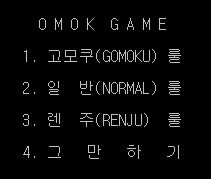
\includegraphics[width=0.5\linewidth]{first.png}
		\end{center}
		\label{fig:long}
		\label{fig:onecol}
	\end{figure}
\begin{center}
		{\Large 룰 선택 화면}
\end{center}




\begin{figure}[h] %%% t: top, b: bottom, h: here
	\begin{center}
		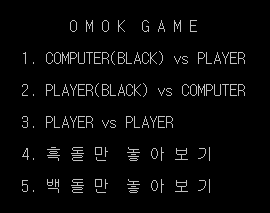
\includegraphics[width=0.5\linewidth]{second.png}
	\end{center}
	\label{fig:long}
	\label{fig:onecol}
\end{figure}
\begin{center}
	{\Large 플레이어 선택 화면}
\end{center}

	\newpage
\begin{figure}[h] %%% t: top, b: bottom, h: here
	\begin{center}
		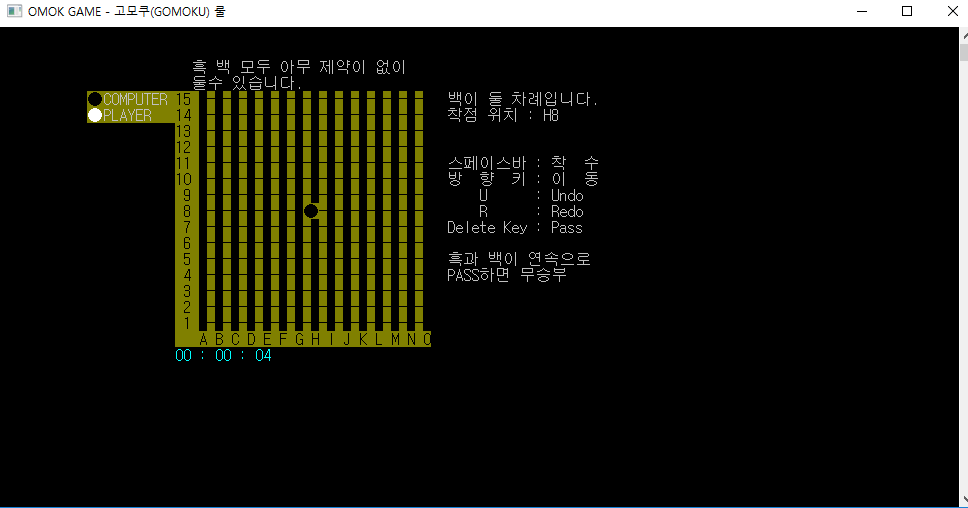
\includegraphics[width=0.8\linewidth]{third.png}
	\end{center}
	\label{fig:long}
	\label{fig:onecol}
\end{figure}
\begin{center}
	{\Large 게임 실행 화면}
\end{center}
\end{document} 